\chapter{\MakeUppercase{Программная архитектура}} \label{chap:arch}
\section{Структура управления}

Высокоуровневая логика запрограммирована на микрокомпьютере \textit{Rasp}-\textit{berry Pi}. Тот в свою очередь отправляет последовательность команд на платформу \textit{Arduino}, которая управляет сервоприводами через специальный драйвер и отправляет информацию о своем состоянии в виде обратной связи на микрокомпьютер. Упрощенная схема реализованной системы приведена на рисунке \ref{fig:upravlenie}.

\begin{figure}[h!]
    \centering
    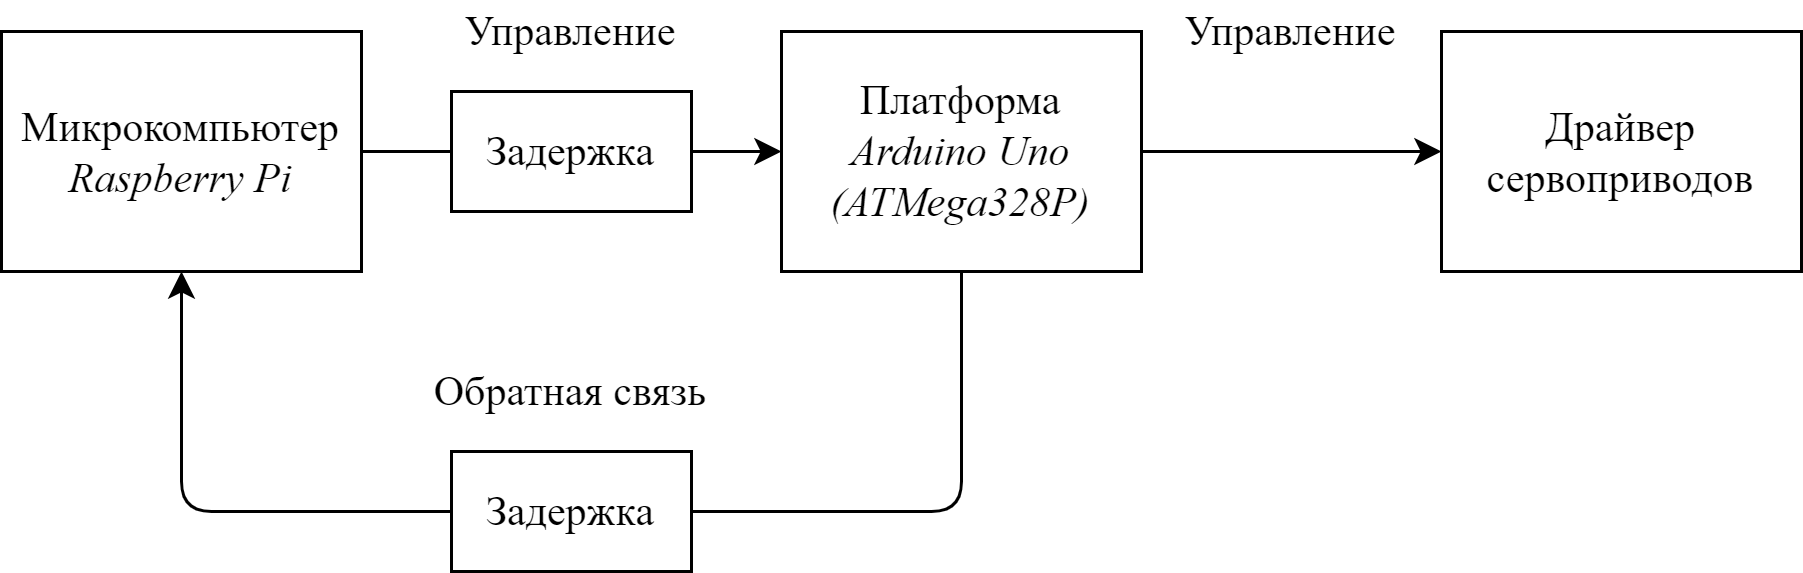
\includegraphics[width=\textwidth]{chapter_arch/figure2.png}
    \caption{Упрощенная схема системы управления робота}
    \label{fig:upravlenie}
\end{figure}

\section{Протокол передачи данных} \label{sec:protocol}
Отправка команд от \textit{Raspberry Pi} к \textit{Arduino} и последующий прием обратной связи производится через интерфейс \textit{Serial}. Это самый надежный вариант при условии, что для установки соединения используется обыкновенный \textit{USB} кабель, который уже защищен от помех и штекер которого надежно закреплен в разъеме.

Для достижения наилучшей скорости реакции микроконтроллера на команды был разработан специальный протокол передачи данных и были написаны легковесные программные библиотеки. Для платформы \textit{Arduino} код написан на языке \textit{C++}, для микрокомпьютера \textit{Raspberry Pi} была разработана библиотека на языке \textit{Python}.

\noindent Библиотека для передачи данных написана для трёх платформ. Она сильно упрощает наладку управления \textit{Arduino} с помощью \textit{Raspberry Pi}. Основная идея программного кода в том, чтобы микрокомпьютер отправлял на микроконтроллер очень простые команды, состоящие из массива байт, в который зашифрованы лишь целочисленный номер и вещественные аргументы. Обратная связь от микроконтроллера реализована в формате \textit{JSON}.

\begin{figure}[h]
    \centering
    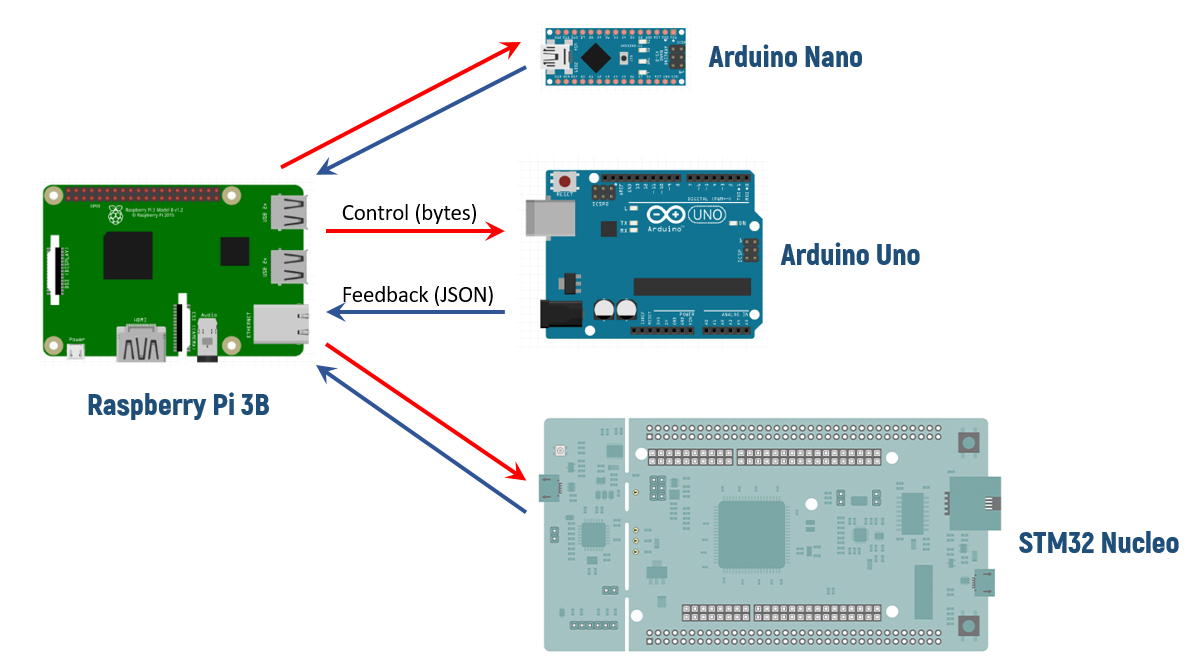
\includegraphics[scale=0.6]{chapter_arch/figure1.png}
    \caption{Управление микроконтроллерами с помощью \textit{Raspberry Pi}}
    \label{}
\end{figure}

\textbf{Для справки}: \textit{JSON} это сокращение от \textit{JavaScript Object Notation} -- формата передачи данных. Как можно понять из названия, \textit{JSON} произошел из \textit{JavaScript}, но он доступен для использования на многих других языках, включая \textit{Python, Ruby, PHP} и \textit{Java}, в англоязычным странах его в основном произносят как \textit{Jason}, то есть как имя Джэйсон. Легкочитаемый и компактный, \textit{JSON} представляет собой хорошую альтернативу \textit{XML} и требует куда меньше форматирования контента \cite{Jayson2018}.

\noindent Объект \textit{JSON} это набор данных в формате <<ключ-значение>>, который находится в фигурных скобках.
Вот так выглядит \textit{JSON} объект:
\begin{code}
{
  "first_name" : "Anton",
  "last_name" : "Kolomeytsev",
  "location" : "Moscow",
  "online" : true,
  "languages" : ["Russian", "English"] 
}
\end{code}

Массив байт, отправляемый на микроконтроллер, всегда имеет одну и ту же структуру, которую легко расшифровать. Каждая команда имеет свой идентификатор (число от 0 до 255), а также может не иметь вовсе, либо иметь ограниченное числом $ 256^4 $ количество аргументов. 

При отправке инструкции на микроконтроллер первым байтом всегда идет номер (идентификатор) команды. Вторым байтом идет число -- количество аргументов. Если у команды нет аргументов, байт нулевой. Пример команды без аргументов с идентификатором $ 207 $:
\begin{equation*}
    \overbrace{11001111}^{идентификатор\: команды} \underbrace{00000000}_{количество\: аргументов}
\end{equation*}

К каждому идентификатору можно привязать выполнение роботом какого-либо действия. Например, включение или выключение компрессора, и т.д. Но бывает, что нужно уточнить параметры выполнения команды какими-то числовыми аргументами. В таком случае второй байт будет ненулевым и он будет указывать на количество идущих после второго байта блоков длиной в 4 байта. В каждом таком четырёхбайтном блоке хранится вещественное число. Пример команды с идентификатором $ 209 $ с одним вещественным аргументом:
\begin{equation*}
    \overbrace{11010001}^{идентификатор\: команды} \underbrace{00000001}_{количество\: аргументов} \overbrace{10110001 \;\; 11100010 \;\; 00110100 \;\; 00100100}^{вещественный \: аргумент}
\end{equation*}

Описанным образом можно реализовать команду, которой передаются, например, требуемые скорости вращения колес, или параметры чувствительности датчиков, и т.д.

Преимущества выбранного подхода:
\begin{itemize}
    \item Микроконтроллер способен очень быстро расшифровать массив байт. Поэтому задержка между отправкой команды и её исполнением для человека не заметна.
    \item Невозможно перенести высокоуровневый функционал и принятие решений на микроконтроллер. Это заставляет продумывать структуру системы.
    \item При таком формате общения между устройствами разработка  укладывается в основы теории автоматического управления.
    \item Возможность подключить до четырёх микроконтроллеров к одному \textit{Raspberry Pi}.
\end{itemize}

\textbf{Протокол}

Правила, по которым устанавливается соединение, следующие:
\begin{itemize}
    \item[1.] \textit{Raspberry Pi} устанавливает соединение с \textit{Arduino} по \textit{USB}, открывая \textit{Serial} порт между устройствами.
    \item[2.] \textit{Arduino} отправляет свой уникальный идентификатор.
    \item[3.] После получения идентификатора \textit{Raspberry} может использовать его для обмена данными. 
\end{itemize}

При написании кода на \textit{Raspberry}, есть всего три простых функции:

\noindent Функция \textit{push}: отправляет команду под номером \textit{CODE} с аргументами \textit{ARG}
\begin{code}
clapi.device_id.push(CODE[, ARG1, ARG2, ..., ARGN])
\end{code}

\noindent Функция \textit{pull}: блокирует выполнение программы, дожидается входящего сообщения от устройства. Возвращает \textit{JSON}, который нам прислало устройство.
\begin{code}
clapi.device_id.pull()
\end{code}

\noindent Функция \textit{request}: отправляет команду как \textit{push}, после чего дожидается ответа как \textit{pull}.
\begin{code}
clapi.device_id.request(CODE[, ARG1, ARG2, ..., ARGN])
\end{code}

Первая версия кода библиотеки для управления была написана автором в 2019 году, использовалась <<в боевых условиях>> и достойно показала себя на робототехнических соревнованиях \textit{Eurobot} \cite{Kekmech2020}. С тех пор код был доработан, дополнительно протестирован и оптимизирован под новые нужды.

\section{Кинематические расчеты}

Перенос расчётов из систем математических расчетов вроде \textit{Matlab, SciLab} или \textit{Mathematica} на один из языков программирования это не всегда тривиальная задача. Самая сложная часть переноса -- матричные вычисления, элементы математического анализа (пределы, производные, интегрирование), решение систем СЛАУ, решение систем нелинейных уравнений. При переносе кинематических расчётов в рамках данного проекта понадобилось реализовать численно следующие функции:
\begin{itemize}
    \item вычисление задачи о положениях;
    \item решение тригонометрической задачи о четырехзвеннике;
    \item вычисление Якобиана;
    \item решение обратной задачи кинематики.
\end{itemize}

Использование библиотеки численной математики \textit{Numpy} на языке программирования \textit{Python} сильно упростило задачу. Стоит отметить, что \textit{Numpy} сегодня активно используется для математических вычислений исследователями всех стран \cite{Numpy2020}.

\subsection{Вычисление задачи о положениях}

Самая простая в реализации задача -- найти три координаты и вернуть вектор:
\begin{python}
def direct(angles):
    phi1, phi2, phi3 = angles[0], angles[1], angles[2]
    phi4 = four_link_angle(phi3) - (pi/2)
    X = A2 + A3 * cos(phi2) + A6 * sin(phi2) + A8 * sin(phi2 + phi4) + (A9 + A10) * cos(phi2 + phi4)
    V = A1 - A3 * sin(phi2) + A6 * cos(phi2) + A8 * cos(phi2 + phi4) - (A9 + A10) * sin(phi2 + phi4)
    Y = V * sin(phi1)
    Z = V * cos(phi1)
    return np.array([X, Y, Z])
\end{python}

\noindent Декомпозируем входные углы, подставляем их в формулы, получая $ X, Y, Z $, и возвращаем вектор $ F^* =[ X, Y, Z ] $.

\subsection{Решение задачи о четырехзвеннике}
Тоже не сложная задача, если есть готовое решение в математическом пакете \textit{Mathematica}.
\begin{python}
def four_link_angle(phi3):
    d = sqrt(A5**2 + A7**2 - 2 * A5 * A7 * cos(phi3 + pi/2))
    gamma = asin((A5 / d) * cos(phi3))
    delta = acos((d**2 + A9**2 - A7**2) / (2 * d * A9))
    return (pi - gamma - delta)
\end{python}

\noindent Вычисления здесь достаточно громоздкие, хотя угол $ \varphi_3 $ не сильно отличается от $ \varphi_4 $.

\subsection{Вычисление Якобиана}
Для численного решения обратной задачи кинематики нужно в каждой итерации вычислять Якобиан. Аналитический вид производной кинематического графа представленной в работе конечности неоправданно больших размеров, что делает невозможным его перенос из математического пакета в код на \textit{Python}. Однако используя функцию вычисляющую прямую задачу кинематики, и устанавливая шаг для приращения каждого угла мы можем дифференцировать численно следующим образом \cite{Morken2010}:
\begin{align*}
    \frac{\partial f}{\partial x}(a, b) &\approx \frac{f(a+h_1, b) - f(a, b)}{h_1}, \\ 
    \frac{\partial f}{\partial y}(a, b) &\approx \frac{f(a, b+h_2) - f(a, b)}{h_2}
\end{align*}

\noindent Можно оценить погрешность вычисления:
\begin{align*}
    \frac{\partial f}{\partial x}(a, b) - \frac{f(a+h_1, b) - f(a, b)}{h_1} &= \frac{h_1}{2} \frac{\partial^2 f}{\partial x^2}(c_1, b), \\ 
    \frac{\partial f}{\partial y}(a, b) - \frac{f(a, b+h_2) - f(a, b)}{h_2} &= \frac{h_2}{2} \frac{\partial^2 f}{\partial y^2}(a, c_2)
\end{align*}
\noindent Где $ c_1 \subset (a, a+h_1) $, а $ с_2 \subset (b, b+c_2) $. Такой результат нас вполне устраивает, поэтому реализация в коде следующая:
\begin{python}
def jacobian(angles):
    h = pi * 1e-4 # diff step
    F = direct(angles)
    eye = np.eye(3) * h # matrix with all h in diagonal elements
    dFdPhi1 = (direct(angles + eye[0]) - F) / h
    dFdPhi2 = (direct(angles + eye[1]) - F) / h
    dFdPhi3 = (direct(angles + eye[2]) - F) / h
    return np.array([dFdPhi1, dFdPhi2, dFdPhi3]).reshape((3, 3)).T
\end{python}

\noindent Для оптимизации вычисления идут сразу по строкам матрицы.
Решение обратной задачи кинематики уже было рассмотрено в пункте \ref{sec:inverse_kin}.

\section{Тестирование кода}

При разработке программной части любого устройства существует непропадающая проблема. Разработчики не могут писать код без ошибок. Более того, в сложных программных системах при внесении каких-либо изменений слишком сложно понять, как это отразится на других частях.

Для того, что бы минимизировать поиски ошибок в коде и ускорить их обнаружение, пишутся так называемые \textit{Unit}-тесты. Такие тесты сами по себе являются программами, но сильно более простыми, чем сама система. Эти тесты автоматически запускаются при внесении в код системы изменений и выводят предупреждения в случае неправильного поведения или логики работы системы.
Автоматические тесты -- это хороший тон в программировании.

В нашем случае, например, тесты запускают функции решающие задачи кинематики с разными входными данными и сверяют ответы с теми числами, которые заранее рассчитаны в \textit{Mathematica}. Если ответы не сходятся (с нужной точностью), нам покажут предупреждение. Таким образом ошибки, которые могли быть внесены в алгоритмы, связанные с кинематическими расчетами, будут выявлены до того, как код будет запущен на физической модели робота. Что повышает безопасность работы с такой системой.

Для тестирования кода на \textit{Raspberry Pi} используется библиотека \textit{PyTest}.

% \section{Абстракция над вычислениями}
